% =====================================================================
% Skeleton D — Vertical 3-Segment + Right Side Panel
% =====================================================================
% USAGE: Adapted from a GOLD STANDARD figure (Privacy-Preserving FL with
% HE & Secure Aggregation). Agent / sub-agent: copy ENTIRE file as figure.tex,
% then change ONLY the content (text/labels/numbers). DO NOT touch:
%   - Zone coordinates (Client Layer / Cryptographic Pipeline / Global Model)
%   - Right side panel position (Security Analysis radar + advantages box)
%   - Bottom chart pair (Convergence + Communication Cost)
%
% LAYOUT MODEL:
%   ┌──────────────────────────────────────┬──────────┐
%   │ Segment 1: top horizontal row        │   Right  │
%   │ (e.g., N parallel clients/inputs)    │   side   │
%   ├──────────────────────────────────────┤  panel   │
%   │ Segment 2: middle pipeline           │ (radar+  │
%   │ (e.g., 3-step crypto / processing)   │  text)   │
%   ├──────────────────────────────────────┴──────────┤
%   │ Segment 3: bottom aggregator + 2 result charts  │
%   └─────────────────────────────────────────────────┘
%
% WHEN TO USE: Federated/distributed system papers, multi-party crypto
% protocols, layered architectures with security/performance analysis.
%
% CONTAINS: 4 parallel clients + 3 pipeline steps with embedded math +
% radar chart + advantages list + 2 bottom charts. Supports 中文/English
% mix (uses ctex + PingFang SC — requires macOS font or substitute).
%
% CONSTRAINTS — DO NOT VIOLATE (each one caused a real layout bug):
%
%   [RENAMING — most common agent / sub-agent failure: leaving stale template labels]
%   - 4 top clients labeled "Client A/B/C/D" — RENAME ALL to match topic
%     (e.g., "Expert 1..4" for MoE, "Worker i" for distributed). Do not
%     leave any "Client X" if the topic is not FL.
%   - 3 zone labels "Client Layer" / "Cryptographic Pipeline" /
%     "Global Model & Evaluation" — RENAME to topic.
%   - "Local SGD η=0.01" residual under client box — RENAME or remove.
%   - Radar 5 axis labels (Privacy/Robustness/Accuracy/Comm/Compute) —
%     RENAME but keep them SHORT (see radar constraint).
%
%   [RADAR CHART — strict label rules]
%   - 270° (bottom) axis label MUST be SINGLE LINE (e.g., "Accuracy").
%     2-line label like "Model\\Accuracy" overlaps the legend at y≈12-13.
%   - Legend fixed at (19.5, 12.0); Advantages box at (19.5, 11.4)
%     anchor=north. If you reposition radar/legend, move advantages too,
%     and extend security zone bottom (currently y=9.0) to match.
%
%   [ARROW + LABEL POSITIONING]
%   - Δw and Enc(Δw) labels go BESIDE arrows (anchor=west/east + ~0.15cm
%     offset), NOT on top of arrows — text-on-arrow overlap.
%   - FedAvg → bottom charts: use DIRECT diagonals. NOT L-shape (-|) when
%     the waypoint y equals the target y — that produces a horizontal
%     arrowhead at the chart top instead of pointing down.
% =====================================================================

\documentclass[tikz,border=25pt]{standalone}
\usepackage{tikz}
\usepackage[fontset=none]{ctex}
\setCJKmainfont{PingFang SC}
\setCJKsansfont{PingFang SC}
\usepackage{amsmath,amssymb}
\usetikzlibrary{shapes, arrows.meta, positioning, fit, backgrounds, calc, shadows, shapes.geometric}

% ===== Academic Palette =====
\definecolor{acaBlueLine}{HTML}{3B82F6}      \definecolor{acaBlueFill}{HTML}{DBEAFE}
\definecolor{acaPurpleLine}{HTML}{7030E0}    \definecolor{acaPurpleFill}{HTML}{EDE9FE}
\definecolor{acaTealLine}{HTML}{009060}      \definecolor{acaTealFill}{HTML}{D1FAE5}
\definecolor{acaGreenLine}{HTML}{30A060}     \definecolor{acaGreenFill}{HTML}{ECFDF5}
\definecolor{acaOrangeLine}{HTML}{F59E0B}    \definecolor{acaOrangeFill}{HTML}{FEF3C7}
\definecolor{acaRedLine}{HTML}{E03030}       \definecolor{acaRedFill}{HTML}{F8CECC}
\definecolor{acaGreyLine}{HTML}{666666}      \definecolor{acaGreyFill}{HTML}{F5F5F5}
% Deep purple variants
\definecolor{purpleDeep}{HTML}{401090}
\definecolor{purpleMid}{HTML}{6020D0}
\definecolor{purpleLight}{HTML}{8B5CF6}
\definecolor{purplePale}{HTML}{C4B5FD}
% Chart
\definecolor{chartBlue}{HTML}{3080C0}
\definecolor{chartGreen}{HTML}{009060}
\definecolor{chartOrange}{HTML}{F59E0B}

\pgfdeclarelayer{background}
\pgfdeclarelayer{deepbg}
\pgfsetlayers{deepbg,background,main}

\begin{document}
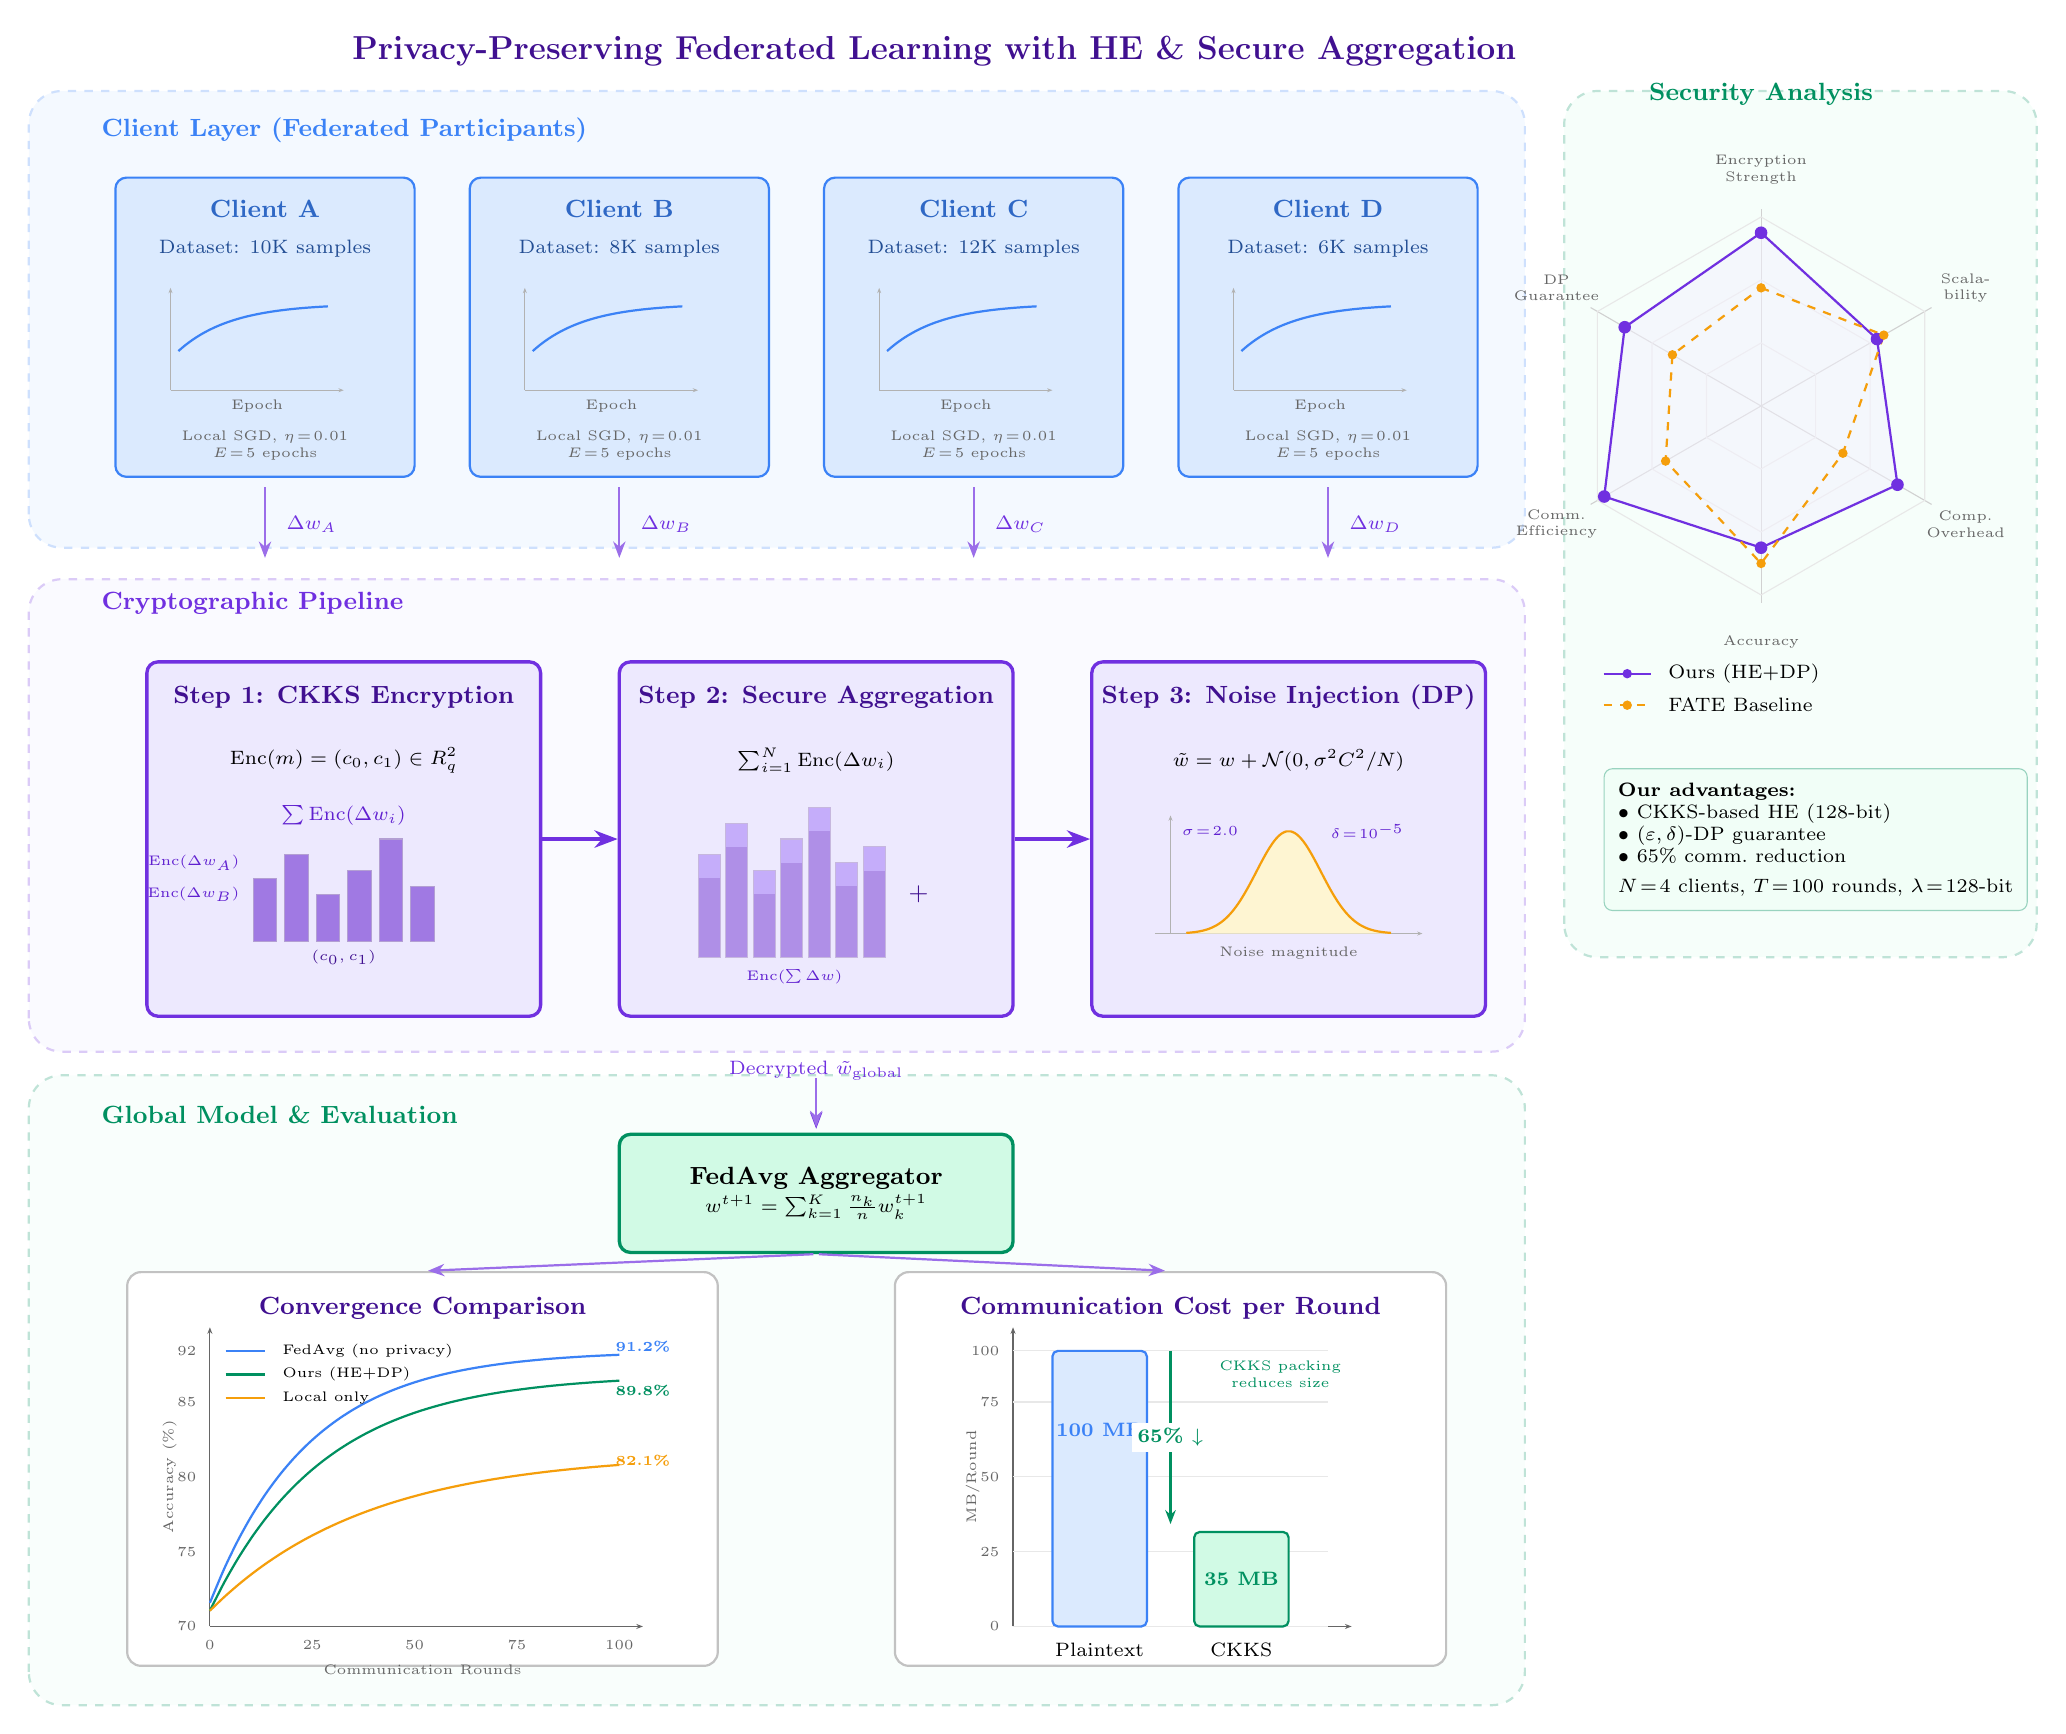
\begin{tikzpicture}[
    every node/.style={font=\small},
    base_box/.style={rectangle, rounded corners=4pt, align=center,
        minimum height=0.8cm, minimum width=2.4cm,
        inner sep=8pt, thick},
    arrow/.style={-{Stealth[scale=0.9]}, thick, color=acaPurpleLine!70, shorten >=2pt, shorten <=1pt},
]

% ================================================================
%  TITLE
% ================================================================
\node[font=\large\bfseries, text=purpleDeep] at (11, 20.5)
    {Privacy-Preserving Federated Learning with HE \& Secure Aggregation};

% ================================================================
%  CLIENT LAYER (top, 4 clients)
% ================================================================
\node[font=\small\bfseries, text=acaBlueLine, anchor=west] at (0.3, 19.5)
    {Client Layer (Federated Participants)};

\foreach \i/\name/\samples/\xc in {A/Client A/10K/2.5, B/Client B/8K/7, C/Client C/12K/11.5, D/Client D/6K/16} {
  % Client box
  \node[base_box, fill=acaBlueFill, draw=acaBlueLine,
        minimum width=3.8cm, minimum height=3.8cm] (client\i) at (\xc, 17.0) {};
  \node[font=\small\bfseries, text=acaBlueLine!80!black] at (\xc, 18.5) {\name};
  \node[font=\scriptsize, text=acaBlueLine!60!black] at (\xc, 18.0) {Dataset: \samples\ samples};

  % Mini training curve inside each client
  \begin{scope}[shift={(\xc-1.2, 16.2)}]
    \draw[-{Stealth[scale=0.4]}, acaGreyLine!50] (0, 0) -- (0, 1.3);
    \draw[-{Stealth[scale=0.4]}, acaGreyLine!50] (0, 0) -- (2.2, 0);
    \draw[acaBlueLine, thick, smooth, samples=30, domain=0.1:2.0]
        plot (\x, {1.1 - 0.7*exp(-1.5*\x)});
    \node[font=\tiny, text=acaGreyLine] at (1.1, -0.2) {Epoch};
  \end{scope}

  % Training params
  \node[font=\tiny, text=acaGreyLine, align=center] at (\xc, 15.5)
      {Local SGD, $\eta\!=\!0.01$\\$E\!=\!5$ epochs};
}

% Arrows from clients down (drawn FIRST so labels sit beside, not on top)
\foreach \xc in {2.5, 7, 11.5, 16} {
  \draw[arrow] (\xc, 15.0) -- (\xc, 14.0);
}

% Delta w labels — placed BESIDE the arrows (anchor=west, +0.15cm right)
% Was at (xc, 14.5) directly on top of the arrow line at the same x.
% Now: label's left edge sits 0.15cm to the right of the arrow.
\node[font=\scriptsize, text=acaPurpleLine, anchor=west] at (2.65, 14.5) {$\Delta w_A$};
\node[font=\scriptsize, text=acaPurpleLine, anchor=west] at (7.15, 14.5) {$\Delta w_B$};
\node[font=\scriptsize, text=acaPurpleLine, anchor=west] at (11.65, 14.5) {$\Delta w_C$};
\node[font=\scriptsize, text=acaPurpleLine, anchor=west] at (16.15, 14.5) {$\Delta w_D$};

% ================================================================
%  CRYPTOGRAPHIC PIPELINE (middle)
% ================================================================
\node[font=\small\bfseries, text=acaPurpleLine, anchor=west] at (0.3, 13.5)
    {Cryptographic Pipeline};

% Step 1: CKKS Encryption
\node[base_box, fill=acaPurpleFill, draw=acaPurpleLine,
      minimum width=5.0cm, minimum height=4.5cm, line width=1.2pt] (ckks) at (3.5, 10.5) {};
\node[font=\small\bfseries, text=purpleDeep] at (3.5, 12.3)
    {Step 1: CKKS Encryption};
\node[font=\scriptsize, align=center] at (3.5, 11.5)
    {$\mathrm{Enc}(m) = (c_0, c_1) \in R_q^2$};
\node[font=\scriptsize, text=purpleMid] at (3.5, 10.8)
    {$\sum \mathrm{Enc}(\Delta w_i)$};

% CKKS cipher blocks visualization
% Fix: 6 bars span 6*0.4=2.4cm (offset 0 to 0+5*0.4+0.3=2.3 actually).
% Bars center should = box center 3.5. xC0 = 3.5 - 1.15 = 2.35
\begin{scope}[shift={(2.35, 9.2)}]
  \foreach \i/\h in {0/0.8, 1/1.1, 2/0.6, 3/0.9, 4/1.3, 5/0.7} {
    \fill[purpleMid!60] ({\i*0.4}, 0) rectangle ({\i*0.4+0.3}, \h);
    \draw[purpleDeep!40, thin] ({\i*0.4}, 0) rectangle ({\i*0.4+0.3}, \h);
  }
  \node[font=\tiny, text=purpleDeep] at (1.15, -0.2) {$(c_0, c_1)$};
\end{scope}

% Enc labels — anchored at the LEFT EDGE of the bar group, extending leftward.
% Was at (2.0, 10.2)/(2.0, 9.8) with default center anchor → text right-edge
% reached x≈2.65, overlapping leftmost bar at x=2.35-2.65.
% Now: anchor=east at x=2.30 (0.05cm left of bars) → text extends leftward,
% safely inside box (left edge x=1.0). No bar overlap.
\node[font=\tiny, text=purpleMid, anchor=east] at (2.30, 10.2) {$\mathrm{Enc}(\Delta w_A)$};
\node[font=\tiny, text=purpleMid, anchor=east] at (2.30, 9.8) {$\mathrm{Enc}(\Delta w_B)$};

% Step 2: Secure Aggregation
\node[base_box, fill=acaPurpleFill, draw=acaPurpleLine,
      minimum width=5.0cm, minimum height=4.5cm, line width=1.2pt] (secagg) at (9.5, 10.5) {};
\node[font=\small\bfseries, text=purpleDeep] at (9.5, 12.3)
    {Step 2: Secure Aggregation};
\node[font=\scriptsize, align=center] at (9.5, 11.5)
    {$\sum_{i=1}^{N} \mathrm{Enc}(\Delta w_i)$};

% Aggregation visualization (stacked bars)
% Fix: 7 bars span 7*0.35=2.45cm with + symbol on right. Group total
% width = bars (2.45) + gap (0.15) + plus (0.4) = 3.0cm.
% Box center=9.5, group should center at 9.5 → xC0 = 9.5 - 1.5 = 8.0
\begin{scope}[shift={(8.0, 9.0)}]
  \foreach \i/\h in {0/1.0, 1/1.4, 2/0.8, 3/1.2, 4/1.6, 5/0.9, 6/1.1} {
    \fill[purpleMid!50] ({\i*0.35}, 0) rectangle ({\i*0.35+0.28}, \h);
    \fill[purpleLight!50] ({\i*0.35}, \h) rectangle ({\i*0.35+0.28}, {\h+0.3});
    \draw[purpleDeep!30, thin] ({\i*0.35}, 0) rectangle ({\i*0.35+0.28}, {\h+0.3});
  }
  % bar group center at x=1.225 within scope
  \node[font=\tiny, text=purpleMid] at (1.225, -0.25) {$\mathrm{Enc}(\sum \Delta w)$};
  % Plus symbol — at right of bars
  \node[font=\small\bfseries, text=purpleDeep] at (2.8, 0.8) {$+$};
\end{scope}

% Step 3: Noise Injection (DP)
\node[base_box, fill=acaPurpleFill, draw=acaPurpleLine,
      minimum width=5.0cm, minimum height=4.5cm, line width=1.2pt] (dp) at (15.5, 10.5) {};
\node[font=\small\bfseries, text=purpleDeep] at (15.5, 12.3)
    {Step 3: Noise Injection (DP)};
\node[font=\scriptsize, align=center] at (15.5, 11.5)
    {$\tilde{w} = w + \mathcal{N}(0, \sigma^2 C^2 / N)$};

% Gaussian bell curve
\begin{scope}[shift={(14.0, 9.3)}]
  \draw[-{Stealth[scale=0.4]}, acaGreyLine!50] (0, 0) -- (0, 1.5);
  \draw[-{Stealth[scale=0.4]}, acaGreyLine!50] (-0.2, 0) -- (3.2, 0);
  \fill[acaOrangeFill!80, smooth, samples=50, domain=0.2:2.8]
      plot (\x, {1.3*exp(-3*(\x-1.5)*(\x-1.5))}) -- (2.8, 0) -- (0.2, 0) -- cycle;
  \draw[acaOrangeLine, thick, smooth, samples=50, domain=0.2:2.8]
      plot (\x, {1.3*exp(-3*(\x-1.5)*(\x-1.5))});
  \node[font=\tiny, text=acaGreyLine] at (1.5, -0.25) {Noise magnitude};
  \node[font=\tiny, text=purpleMid] at (0.5, 1.3) {$\sigma\!=\!2.0$};
  \node[font=\tiny, text=purpleMid] at (2.5, 1.3) {$\delta\!=\!10^{-5}$};
\end{scope}

% Step connections (Fix D.1: removed wrong (secagg.east → dp.east) arrow
% and stale "Fix" comments; only the correct ones are kept)
\draw[-{Stealth[scale=1.0]}, very thick, acaPurpleLine] (ckks.east) -- (secagg.west);
\draw[-{Stealth[scale=1.0]}, very thick, acaPurpleLine] (secagg.east) -- (dp.west);

% Decrypted output label — Fix D.2: was floating in 0.3cm zone gap
% (Crypto bottom y=7.8 / Global top y=7.5). Anchor label to Crypto bottom
% so it visually belongs to the pipeline transition; arrow ends on FedAvg
% box top instead of floating in empty space.
\node[font=\scriptsize, text=acaPurpleLine, anchor=north]
    at (9.5, 7.8) {Decrypted $\tilde{w}_{\text{global}}$};
% Use hard-code coord (fedavg defined later in file — no forward ref)
% fedavg at (9.5, 6.0), height 1.5 → top y=6.75
\draw[arrow, acaPurpleLine] (9.5, 7.5) -- (9.5, 6.75);

% ================================================================
%  SECURITY ANALYSIS (top-right, radar chart)
% ================================================================
% Title anchored center, placed clearly above radar — avoids overlap
% with the Strength axis label which sits at the 90° (top) of the radar.
\node[font=\small\bfseries, text=acaTealLine, anchor=south] at (21.5, 19.7)
    {Security Analysis};

% Radar chart (6 axes)
\begin{scope}[shift={(21.5, 16.0)}]
  % 6 axes
  % Note: 270° label was "Model\\Accuracy" (2-line); shortened to single-line
  % "Accuracy" because the 2-line version spans y=12.83..13.17 and overlaps
  % with the legend's "FATE Baseline" label at y=13.1..13.3 below.
  \foreach \a/\label/\r in {90/Encryption\\Strength/2.2, 30/Scala-\\bility/1.7, 330/Comp.\\Overhead/2.0, 270/Accuracy/1.8, 210/Comm.\\Efficiency/2.3, 150/DP\\Guarantee/2.0} {
    \draw[acaGreyLine!30, thin] (0,0) -- (\a:2.5);
    \node[font=\tiny, text=acaGreyLine, align=center] at (\a:3.0) {\label};
  }
  % Grid rings
  \foreach \ring in {0.8, 1.6, 2.4} {
    \draw[acaGreyLine!15, thin] (90:\ring) -- (30:\ring) -- (330:\ring)
        -- (270:\ring) -- (210:\ring) -- (150:\ring) -- cycle;
  }
  % Ours (purple filled polygon)
  \fill[acaPurpleFill!60, opacity=0.5]
      (90:2.2) -- (30:1.7) -- (330:2.0) -- (270:1.8) -- (210:2.3) -- (150:2.0) -- cycle;
  \draw[acaPurpleLine, thick]
      (90:2.2) -- (30:1.7) -- (330:2.0) -- (270:1.8) -- (210:2.3) -- (150:2.0) -- cycle;
  % Baseline (orange dashed polygon)
  \draw[acaOrangeLine, thick, dashed]
      (90:1.5) -- (30:1.8) -- (330:1.2) -- (270:2.0) -- (210:1.4) -- (150:1.3) -- cycle;
  % Dots on vertices
  \foreach \a/\r in {90/2.2, 30/1.7, 330/2.0, 270/1.8, 210/2.3, 150/2.0} {
    \fill[acaPurpleLine] (\a:\r) circle (0.08);
  }
  \foreach \a/\r in {90/1.5, 30/1.8, 330/1.2, 270/2.0, 210/1.4, 150/1.3} {
    \fill[acaOrangeLine] (\a:\r) circle (0.06);
  }
\end{scope}

% Legend for radar — moved DOWN from (19.5, 13.0) to (19.5, 12.0) so the
% top entry "Ours (HE+DP)" at abs y=12.6 clears the Accuracy axis label
% at y=13.0 (single-line, spans 12.9..13.1) by 0.2cm.
\begin{scope}[shift={(19.5, 12.0)}]
  \draw[acaPurpleLine, thick] (0, 0.6) -- (0.6, 0.6);
  \fill[acaPurpleLine] (0.3, 0.6) circle (0.06);
  \node[font=\scriptsize, anchor=west] at (0.7, 0.6) {Ours (HE+DP)};
  \draw[acaOrangeLine, thick, dashed] (0, 0.2) -- (0.6, 0.2);
  \fill[acaOrangeLine] (0.3, 0.2) circle (0.06);
  \node[font=\scriptsize, anchor=west] at (0.7, 0.2) {FATE Baseline};
\end{scope}

% Advantages box — moved DOWN from y=12.2 to y=11.4 to clear the
% repositioned legend (FATE Baseline bottom at y≈12.1). Box height ~2.06cm
% so new bottom y≈9.34, requires zone bottom ≤ 9.0 for margin.
\node[rectangle, rounded corners=3pt, draw=acaTealLine!40, fill=acaTealFill!30,
      align=left, inner sep=5pt, font=\scriptsize, anchor=north west] at (19.5, 11.4)
    {\textbf{Our advantages:}\\
     $\bullet$ CKKS-based HE (128-bit)\\
     $\bullet$ $(\varepsilon, \delta)$-DP guarantee\\
     $\bullet$ 65\% comm.\ reduction\\[3pt]
     $N\!=\!4$ clients, $T\!=\!100$ rounds, $\lambda\!=\!128$-bit};
% Bottom param line: \quad×2 spacing pushed box right-edge to x≈25.19,
% overflowing zone right edge x=25.0. Replaced \quad with comma+space
% (~0.27cm narrower per gap) so box right edge sits at x≈24.55 with
% 0.45cm margin to zone edge.

% ================================================================
%  GLOBAL MODEL & EVALUATION (bottom)
% ================================================================
\node[font=\small\bfseries, text=acaTealLine, anchor=west] at (0.3, 7.0)
    {Global Model \& Evaluation};

% FedAvg Aggregator
\node[base_box, fill=acaTealFill, draw=acaTealLine, line width=1.2pt,
      minimum width=5.0cm, minimum height=1.5cm] (fedavg) at (9.5, 6.0)
    {\textbf{FedAvg Aggregator}\\[-1pt]{\scriptsize $w^{t+1} = \sum_{k=1}^{K} \frac{n_k}{n} w_k^{t+1}$}};

\draw[arrow] (9.5, 7.5) -- (fedavg.north);

% --- Convergence Comparison (line chart) ---
\node[rectangle, rounded corners=5pt, draw=acaGreyLine!40, fill=white,
      minimum width=7.5cm, minimum height=5.0cm, thick] (conv_box) at (4.5, 2.5) {};
\node[font=\small\bfseries, text=purpleDeep, anchor=north] at (4.5, 4.8)
    {Convergence Comparison};

\begin{scope}[shift={(1.5, 0.5)}]
  % Axes
  \draw[-{Stealth[scale=0.5]}, acaGreyLine] (0.3, 0) -- (0.3, 3.8);
  \draw[-{Stealth[scale=0.5]}, acaGreyLine] (0.3, 0) -- (5.8, 0);
  \node[font=\tiny, text=acaGreyLine, rotate=90, anchor=south] at (0.0, 1.9) {Accuracy (\%)};
  \node[font=\tiny, text=acaGreyLine] at (3.0, -0.55) {Communication Rounds};
  % Y ticks
  \foreach \y/\lab in {0.0/70, 0.95/75, 1.9/80, 2.85/85, 3.5/92} {
    \node[font=\tiny, left, text=acaGreyLine] at (0.25, \y) {\lab};
  }
  % X ticks
  \foreach \x/\lab in {0.3/0, 1.6/25, 2.9/50, 4.2/75, 5.5/100} {
    \node[font=\tiny, below, text=acaGreyLine] at (\x, -0.05) {\lab};
  }
  % Line 1: FedAvg (no privacy) — blue, highest
  \draw[acaBlueLine, thick, smooth, samples=30, domain=0.3:5.5]
      plot (\x, {3.5 - 3.2*exp(-0.8*(\x-0.3))});
  % Line 2: Ours (HE+DP) — teal, middle
  \draw[acaTealLine, thick, smooth, samples=30, domain=0.3:5.5]
      plot (\x, {3.2 - 3.0*exp(-0.7*(\x-0.3))});
  % Line 3: Local only — orange, lowest
  \draw[acaOrangeLine, thick, smooth, samples=30, domain=0.3:5.5]
      plot (\x, {2.2 - 2.0*exp(-0.5*(\x-0.3))});
  % End labels
  \node[font=\tiny\bfseries, text=acaBlueLine] at (5.8, 3.55) {91.2\%};
  \node[font=\tiny\bfseries, text=acaTealLine] at (5.8, 3.0) {89.8\%};
  \node[font=\tiny\bfseries, text=acaOrangeLine] at (5.8, 2.1) {82.1\%};
  % Legend
  \draw[acaBlueLine, thick] (0.5, 3.5) -- (1.0, 3.5);
  \node[font=\tiny, anchor=west] at (1.1, 3.5) {FedAvg (no privacy)};
  \draw[acaTealLine, thick] (0.5, 3.2) -- (1.0, 3.2);
  \node[font=\tiny, anchor=west] at (1.1, 3.2) {Ours (HE+DP)};
  \draw[acaOrangeLine, thick] (0.5, 2.9) -- (1.0, 2.9);
  \node[font=\tiny, anchor=west] at (1.1, 2.9) {Local only};
\end{scope}

% --- Communication Cost per Round (bar chart) ---
\node[rectangle, rounded corners=5pt, draw=acaGreyLine!40, fill=white,
      minimum width=7.0cm, minimum height=5.0cm, thick] (comm_box) at (14, 2.5) {};
\node[font=\small\bfseries, text=purpleDeep, anchor=north] at (14, 4.8)
    {Communication Cost per Round};

\begin{scope}[shift={(11.5, 0.5)}]
  % Axes
  \draw[-{Stealth[scale=0.5]}, acaGreyLine] (0.5, 0) -- (0.5, 3.8);
  \draw[-{Stealth[scale=0.5]}, acaGreyLine] (0.5, 0) -- (4.8, 0);
  \node[font=\tiny, text=acaGreyLine, rotate=90, anchor=south] at (0.2, 1.9) {MB/Round};
  % Y ticks
  \foreach \y/\lab in {0.0/0, 0.95/25, 1.9/50, 2.85/75, 3.5/100} {
    \node[font=\tiny, left, text=acaGreyLine] at (0.45, \y) {\lab};
    \draw[acaGreyLine!15, thin] (0.5, \y) -- (4.5, \y);
  }
  % Plaintext bar (tall, grey-blue)
  \fill[acaBlueFill, draw=acaBlueLine, rounded corners=2pt, thick]
      (1.0, 0) rectangle (2.2, 3.5);
  \node[font=\scriptsize\bfseries, text=acaBlueLine] at (1.6, 2.5) {100 MB};
  \node[font=\scriptsize] at (1.6, -0.3) {Plaintext};
  % CKKS bar (short, teal)
  \fill[acaTealFill, draw=acaTealLine, rounded corners=2pt, thick]
      (2.8, 0) rectangle (4.0, 1.2);
  \node[font=\scriptsize\bfseries, text=acaTealLine] at (3.4, 0.6) {35 MB};
  \node[font=\scriptsize] at (3.4, -0.3) {CKKS};
  % Reduction annotation
  \draw[-{Stealth[scale=0.6]}, very thick, acaTealLine] (2.5, 3.5) -- (2.5, 1.3);
  \node[font=\scriptsize\bfseries, text=acaTealLine, fill=white, inner sep=2pt]
      at (2.5, 2.4) {65\% $\downarrow$};
  % CKKS packing annotation — needs align=center for \\ linebreak
  \node[font=\tiny, text=acaTealLine, anchor=west, align=center] at (3.0, 3.2)
      {CKKS packing\\reduces size};
\end{scope}

% FedAvg → Charts
% Fix: previous L-shape (fedavg.south) -- (9.5, 5.0) -| (chart.north) had
% waypoint (9.5, 5.0) at the SAME y as chart.north (5.0), so the `-|`
% vertical segment had zero length → arrowheads ended HORIZONTALLY at the
% top-edge of each chart (looked like flying arrows / 飞线). With only
% 0.25cm vertical gap between fedavg.south (5.25) and chart.north (5.0),
% no proper L-shape fits. Replaced with direct diagonal lines from
% fedavg.south to each chart's north anchor — arrowheads now land cleanly
% on the chart top, pointing mostly downward.
\draw[arrow] (fedavg.south) -- (conv_box.north);
\draw[arrow] (fedavg.south) -- (comm_box.north);

% ================================================================
%  ZONE BACKGROUNDS
% ================================================================
\begin{pgfonlayer}{deepbg}
  % Client zone (blue)
  \fill[acaBlueFill!30, rounded corners=12pt] (-0.5, 14.2) rectangle (18.5, 20.0);
  \draw[acaBlueLine!25, dashed, thick, rounded corners=12pt] (-0.5, 14.2) rectangle (18.5, 20.0);
  % Crypto zone (purple)
  \fill[acaPurpleFill!25, rounded corners=12pt] (-0.5, 7.8) rectangle (18.5, 13.8);
  \draw[acaPurpleLine!25, dashed, thick, rounded corners=12pt] (-0.5, 7.8) rectangle (18.5, 13.8);
  % Security zone (teal) — extended bottom from 11.5 to 9.0 to contain
  % the "Our advantages" box. Box anchored north-west at (19.5, 11.4),
  % height ≈ 2.06cm → bottom y ≈ 9.34. Zone bottom at 9.0 gives 0.34cm
  % margin below the box.
  \fill[acaTealFill!20, rounded corners=12pt] (19.0, 9.0) rectangle (25.0, 20.0);
  \draw[acaTealLine!25, dashed, thick, rounded corners=12pt] (19.0, 9.0) rectangle (25.0, 20.0);
  % Global zone (green)
  \fill[acaGreenFill!30, rounded corners=12pt] (-0.5, -0.5) rectangle (18.5, 7.5);
  \draw[acaTealLine!25, dashed, thick, rounded corners=12pt] (-0.5, -0.5) rectangle (18.5, 7.5);
\end{pgfonlayer}

% Fix D.3: removed two stub 0.4cm dashed lines at (0,14.2)/(18,14.2)
% that connected nothing — pure visual noise.
% Fix D.1: removed duplicate (secagg.east) -- (dp.west) arrow
% (now drawn once in the "Step connections" block above).

\end{tikzpicture}
\end{document}
